\documentclass[conference]{IEEEtran}
\usepackage{amsmath,amssymb,amsfonts}
\usepackage{algorithmic}
\usepackage{graphicx}
\usepackage{textcomp}
\usepackage{xcolor}

\usepackage{notoccite}
\usepackage[numbers]{natbib}
\usepackage{url}
\def\BibTeX{{\rm B\kern-.05em{\sc i\kern-.025em b}\kern-.08em
    T\kern-.1667em\lower.7ex\hbox{E}\kern-.125emX}}


\begin{document}
\title{A Survey on Hardware Accelerators for Neural Networks}
\author{
\IEEEauthorblockN{Pierre Brosemer}
\IEEEauthorblockA{uitxj@student.kit.edu}
}

\maketitle

\begin{abstract}
This will be my Abstract in \LaTeX.
I am going to write this when I have almost finished the essay since it will probably be easier to give an overview over the topic once the full paper is finished.
The availability of efficient hardware was one of the key factors, which lead to the rise of Neural Network \cite{historyfpgas}. 
\\
\end{abstract}

\section{Introduction}
Artifical Neural Networks (more often Neural Networks) are one of the most promising technologies in the current era of computer science. Neural Networks can be deployed in an enourmous variety of categories and have shown major improvements in these categories, most prominently in Speech and Image Recognition \cite{speech_recognition1} that exceeded prior methods. The field of Artifical Intelligence covers a wide variety of concepts. This paper will mainly cover the subcategory of Deep Learning, more specifically Neural Networks, which falls under the category of Machine Learning. 
\\
Neural Networks are at it's core a very broad simplification of the biological brain consisting of many interconnected neurons, called nodes in Neural Networks. The nodes in a Neural Network are  arranged in different layers. Each node passes on a weighted value to a node in the next layer. If this value is above a certain threshhold the node will be activated. By changing the weights of each node a learning process similiar to that of their biological counterpart is simulated \cite{nn_basics}.
\begin{figure}[h]
	\caption{Typical representation of a Neural Network}
	\centering
	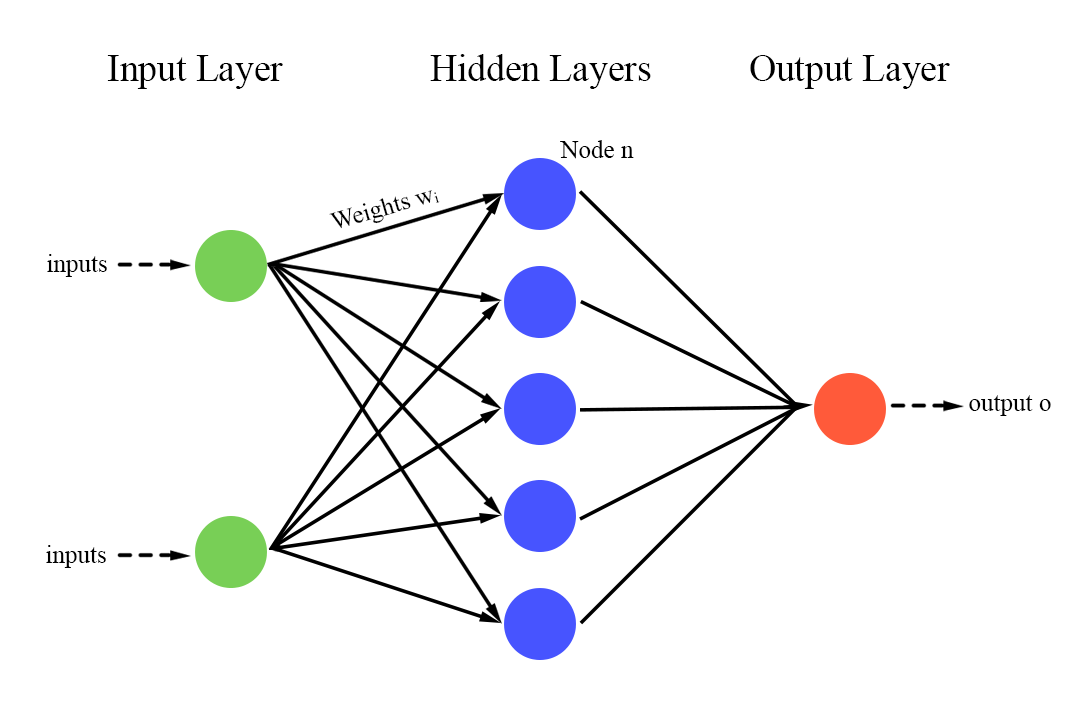
\includegraphics[width=\linewidth]{pictures/neuralnetwork.png}
\end{figure}

The development of a Neural Network consists of two different stages. Firstly a training phase where the Neural Network gets an input and compares the resulting output (prediction) with that of a real-world dataset. The error can then be incorparated into the network by changing the different weights, also called backpropagation. Secondly an inference phase, where the network get's an input and makes a prediction. The Neural Network has a larger computational effort in the training phase as more data is processed, aswell as the weights needing calibration.
\\
\\
With some Neural Networks having over 150 layers \cite{densely_network} up to billions of Multiplications can take place in a single Neural Network. The vast amount of computational power needed for training and using neural network lead to the need for specialised hardware, which contributed much to the success seen in modern day implementations. The research on hardware is still ongoing and is one of the most important topics in achieving better and faster results for Neural Networks. As a result of the timeliness of the topic this survey will only cover a status quo of the current Hardware.
\\

\section{Different Types of Hardware}
Most of Computations needed for inference and training include Matrix-Vector Products, caused by the input data being run through the network.
Furthermore  dimension of the input data plays a key role in the amount of computation needed. A single image can have 1000 pixels resulting in 1000 different data points that the Neural Network has to compute. To efficiently compute the vast amount of data fast memory accesses or inplace computations of the values is needed. Since these Calculations need to be done for the number of nodes good parallelization is needed to efficiently run Neural Networks.
\\
Hardware Accelerators for Neural Networks can be divided into 4 main classes: CPUs, GPUs, FPGAs and ASICs. The focus can be placed on the latter 3 since CPUs mostly fall short in terms of computational power for Neural Networks. 
CPUs are needed for a wide variety of tasks requiring a flexible system to execute instructions. As a result a CPU is good at executing serial instructions in parallel, resulting in a good general parallelization.
Both of the points mentioned above, that are needed for the specialised hardware for Neural Networks, are not met for CPUs. They are limited by their small amount of cores hindering the ability to parallelize the same instruction. Moreover a CPU usually works by fetching an instruction and executing it making the training and inference phase slow \cite{capra2020updated}. While working on Neural Networks CPUs are accompanied by Underutilization, achieving factors of less than 1/10 of that other alternatives \cite{nurvitadhi2016accelerating}.
\\

\section{Graphics Processing Unit}


\newpage
\quad
\newpage

\bibliographystyle{ieeetr}
\bibliography{References}
\end{document}
